% \documentclass[12pt, oneside]{book}

\chapter{Tides}

\label{ch:tides}
\begin{tabular}{ll}
    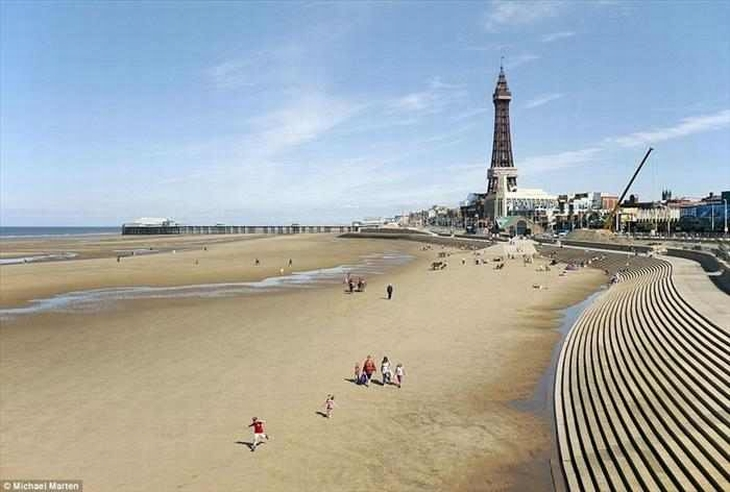
\includegraphics[width=3.2in]{figs/Waves/LowTide.jpg} & 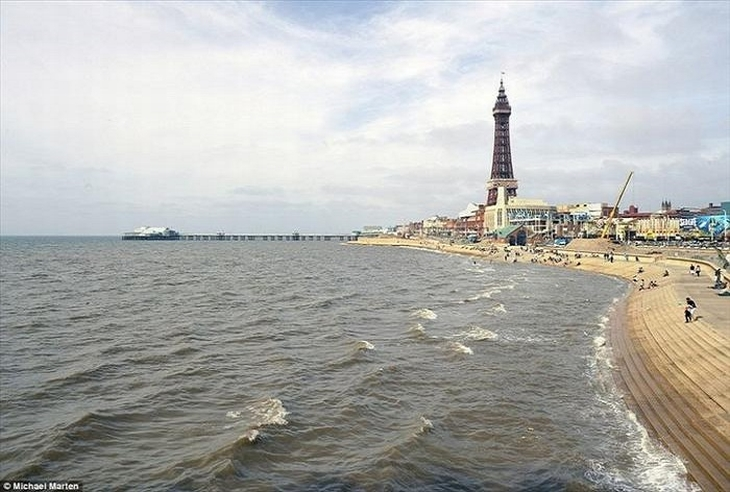
\includegraphics[width=3.2in]{figs/Waves/HighTide.jpg}
\end{tabular}

Tides are an important ocean phenomena. In many places in the ocean they are the dominant source of ocean currents, and we have briefly touched on the fact that they drive mixing in both estuaries and the global ocean.  Here we briefly describe how the various tides arise due to astronomical forcing, and discuss how they manifest in the real ocean.  

Tides are generally caused by the co-orbiting of the moon and the earth, and the earth and the sun.  These orbits cause gravity and centrifugal forces to act on the ocean, and the ocean responds to the forcing with a relatively complex set of waves that move around ocean basins.  Ultimately such waves can only be predicted numerically, but the basic idea behind the forcing can be easily understood.  

\section{Tidal example and describing tides}

A (somewhat) typical tidal signal is shown in \fref{fig:TidePR}.  There are approximately two high tides a day, one is usually higher than the other.  The high tides are move later in the day, indicating that their period is greater than 12 h.  The amplitude of the tide also modulates over the 8 days shown here, with the tidal amplitudes large at the beginning of the time period and becoming more modest towards the end of the time period.  Note that there was a full moon on 1 August.  

\begin{figure}[hbt]
  \begin{center}
    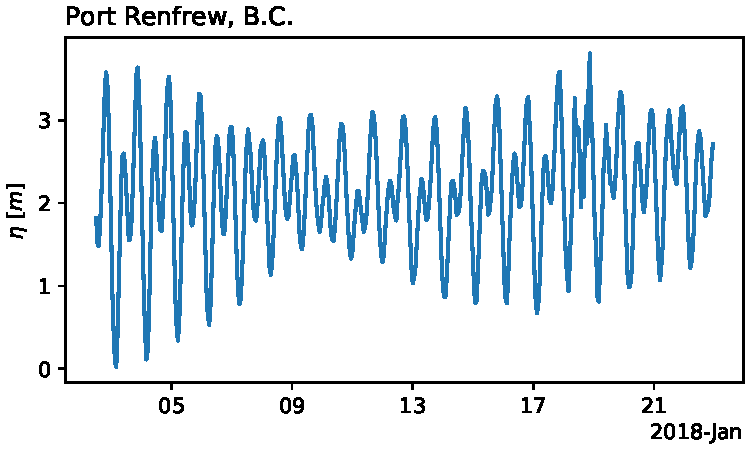
\includegraphics{figs/Waves/TidesRenfrew}
    \caption{Tides observed at Port Renfrew, BC.  }
    \label{fig:TideRenfrew}  
  \end{center}
\end{figure}

When discussing tides it is natural to use the language of waves we saw in the previous chapter (\fref{chap:SurfaceWaves}).  We saw that if we add two waves together of different wavelengths or frequencies we will get an interference pattern.  Using that, we can fit a tidal signal to frequencies we expect from the astronomical forcing, and combine them with the proper amplitude and phase to get a tidal prediction into the future (\fref{fig:FitRenfrew}).

\begin{figure}[hbt]
  \begin{center}
    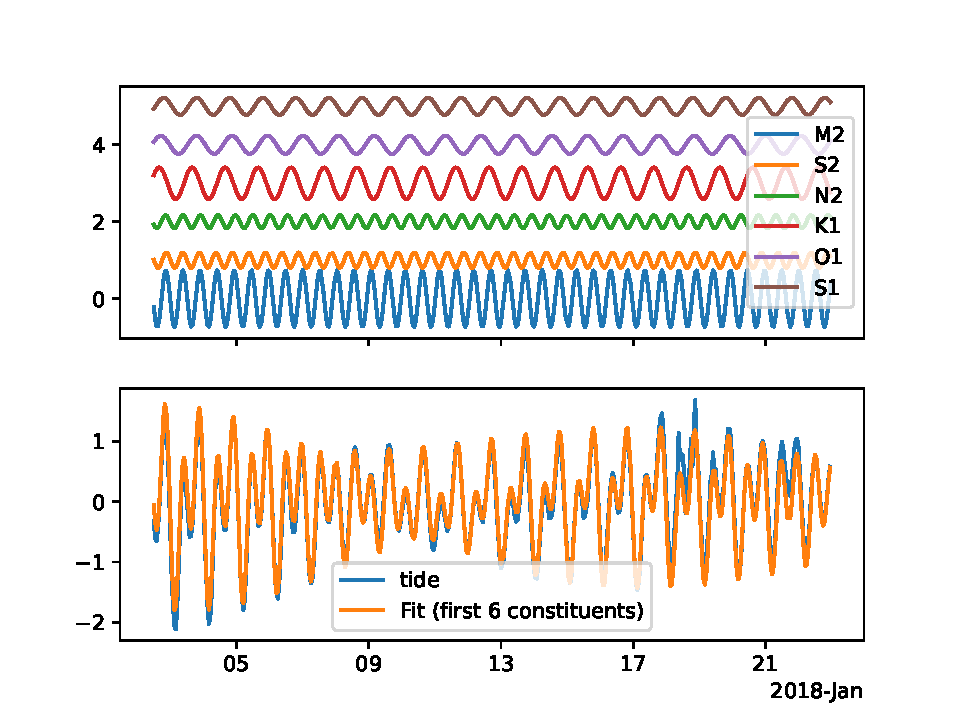
\includegraphics{figs/Waves/FitRenfrew}
    \caption{Harmonic fit of tides at  Port Renfrew, BC.  Upper panel are 6 tidal harmonics with their amplitude and phase fit to the signal in \fref{fig:TideRenfrew}.  Lower panel is the original signal (blue) and the fit (orange).}
    \label{fig:FitRenfrew}  
  \end{center}
\end{figure}

The tides are dominated by frequencies that represent the \emph{semi-dirunal} tides, which are twice a day, and \emph{diurnal} tides, which are once a day (\fref{tab:TideConst}).  In general, it is the interference of $M_2$ and $N_2$, for instance, which give a substantial portion of the spring-neap cycle.  

\begin{figure}[hbt]
  \begin{tabular}{l|ccl}
     & period (h) & Fit at PR (m) & Origin \\
    \hline\hline
    $M_2$ & 12.421 & 0.74 & Principal lunar semidiurnal\\
    $S_2$ & 12.000 & 0.20 & Principal solar semidiurnal\\
    $N_2$ & 12.658 & 0.17 & Larger lunar elliptic semidiurnal\\\hline
    $K_1$ & 23.934 & 0.41 & Lunar diurnal\\
    $O_1$ & 25.819 & 0.24 & Lunar diurnal\\
    $S_1$ & 24.000 & 0.22 & Solar diurnal\\
  \end{tabular}
  \caption{First 6 tidal constituents, and their amplitude at Port Renfrew BC.  }
  \label{tab:TideConst}
\end{figure}



\section{Tidal forces: Gravity and centrifugal forces on co-orbiting bodies}

The tides are driven by the fact that the earth and the moon orbit around one another and the sun and the earth orbit around each other. We usually think of the moon orbiting around the earth every 27.3 days, but the earth also orbits around the center of mass of the earth-moon system every 27.3 days. The point they both orbit around is called the \Wikiref{barycenter}, and for the earth and the moon, it is 4670 km from the center of the earth, which is less than the radius of the earth, so the orbit causes the earth to wobble.  

The earth moves around this barycenter maintaining its orientation in space. This  is shown schematically in \fref{fig:coorbit}, where we have used squares instead of circles to represent the bodies, because it helps makes the orientation of the earth relative to the barycenter.  In each frame, the green dot points "up". Hence the green dot traces exactly the same size circles as the red dot and the center of mass of the earth. Note that the moon behaves differently.  The same face is always angled towards the earth, so that face will make a smaller circle, and the far face will make a larger one.  This phenomena is called \Wikiref{tidal locking} and is why we only see one side of the moon.  

\begin{figure}[hbtp]
  \begin{center}
    \includegraphics[width=2.1in,trim=80 40 80 20,clip]{/Users/jklymak/Eos314/scripts/MoonEarthMovie/pic0000.jpg}
    \includegraphics[width=2.1in,trim=80 40 80 20,clip]{/Users/jklymak/Eos314/scripts/MoonEarthMovie/pic0168.jpg}
    \includegraphics[width=2.1in,trim=80 40 80 20,clip]{/Users/jklymak/Eos314/scripts/MoonEarthMovie/pic0396.jpg}
    \includegraphics[width=2.1in,trim=80 40 80 20,clip]{/Users/jklymak/Eos314/scripts/MoonEarthMovie/pic0552.jpg}
    \caption{Schematic of a square earth co-rotating around its barycenter. with a square moon.  The orbits of two points on the earth are also shown with red and green circles, as is the center of mass of the earth (orange line) and the moon (blue line).  }
    \label{fig:coorbit}
  \end{center}
\end{figure}

The fact that the earth maintains the same orientation in space during its orbit around the barycenter means that every point on the planet feels an identical \Wikiref{centrifugal force}.  This acceleration tends to fling particles away from the axis of rotation with a value 
\begin{equation}
  a_c = \omega^2 r
\end{equation}
where $\omega = 2\pi / 27.3d$ and $r=4670\ \mathrm{km}$ is the distance from th center of the earth to the moon-earth barycenter, so this acceleration in $3.3\times10^{-5}\ \mathrm{m/s^2}$.  

At the center of mass of the earth, this centrifugal acceleration is balanced by the force of gravity of the moon, pulling the earth towards it.  This acceleration is given by Newton's law of universal gravitation:
\begin{equation}
  a_g = \frac{G m_{moon}}{R^2}
\end{equation}
where $G$ is a constant, $m_{moon}$ the mass of the moon, and $R$ the distance from the moon's center of mass to any point on (or in) the earth. 

So the centrifugal force, $a_c$, is the same everywhere on the earth, but the gravitational attraction due to the moon is definitely not, because $R$ varies over the earth, so that points further from the moon experience less gravitational pull than points closer (\fref{fig:TidalForces}).  In addition, points on the earth that are not on the earth-moon axis are pulled towards that axis.  The net effect is that the earth bulges towards \emph{and} \emph{away} from the moon.  

\begin{figure}[hbtp]
  \begin{center}
    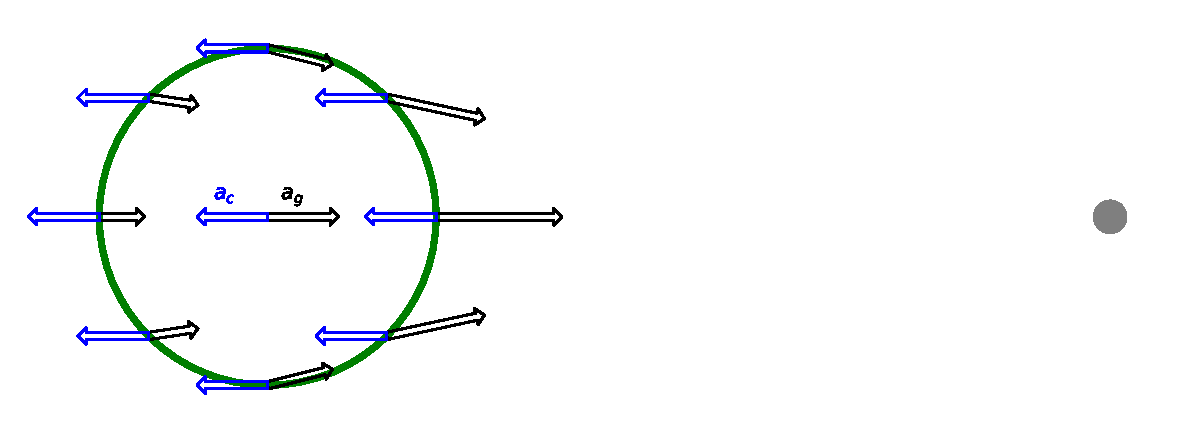
\includegraphics[]{figs/Waves/TidalForces0}
    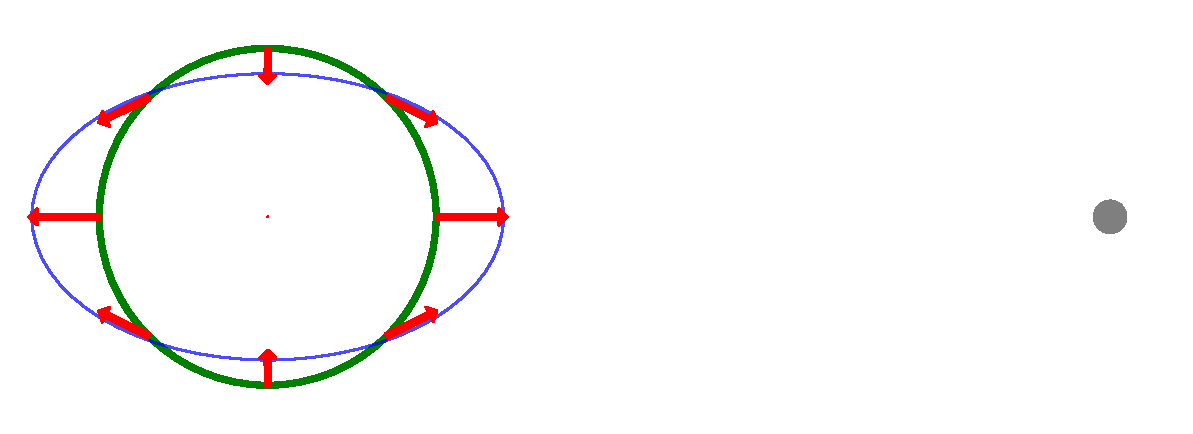
\includegraphics[]{figs/Waves/TidalForces}
    \caption{Sketch of Net tidal forces on earth due to moon. Centrifugal accelerations are shown in blue, and are the same everywhere.  Gravitational accelerations are shown in black, and vary with the inverse square of distance from the moon, and point towards it.  The bottom panel shows the direction of the net forces when the satellite is very far away and a schematic of the tendency of the earth to bulge toward and away from the satellite.   }
    \label{fig:TidalForces}
  \end{center}
\end{figure}

\clearpage 
\clearpage 

\begin{derivbox}[label={box:volumeintegral}]{Centrifugal force}
  The centrifugal force is an \emph{apparent} force (a term I prefer to ``fictitious'') that arises when a co-ordinate system is rotating.  Consider a counter-clockwise rotating system as shown below.  At the first arrow, an object orbiting in the co-ordinate system is moving with speed $\omega R$, where $\omega = 2\pi/T$ is the rotation frequency of the rotating system and $R$ is the distance to the axis of rotation.  The direction that this particle is moving is tangential to the arc of the circle.  
  
If there were no forces acting on the particle at this point, it would travel in a straight line tangential to the circle (along the arrow).  A particle that travelled with the circle would still be on the orbit and would be travelling in a different direction (with the same speed) since the circle bends.  Thus the particle with no external forces is accelerated away from the axis of rotation, and we call this acceleration the ``centrifugal force''.  In order for a particle to continue to move in a circle, there has to be compensating \Wikiref{Centripetal force} pulling the particle towards the axis of rotation.  If the particle were the moon, the centripetal force would be provided by the earth's gravity. 

  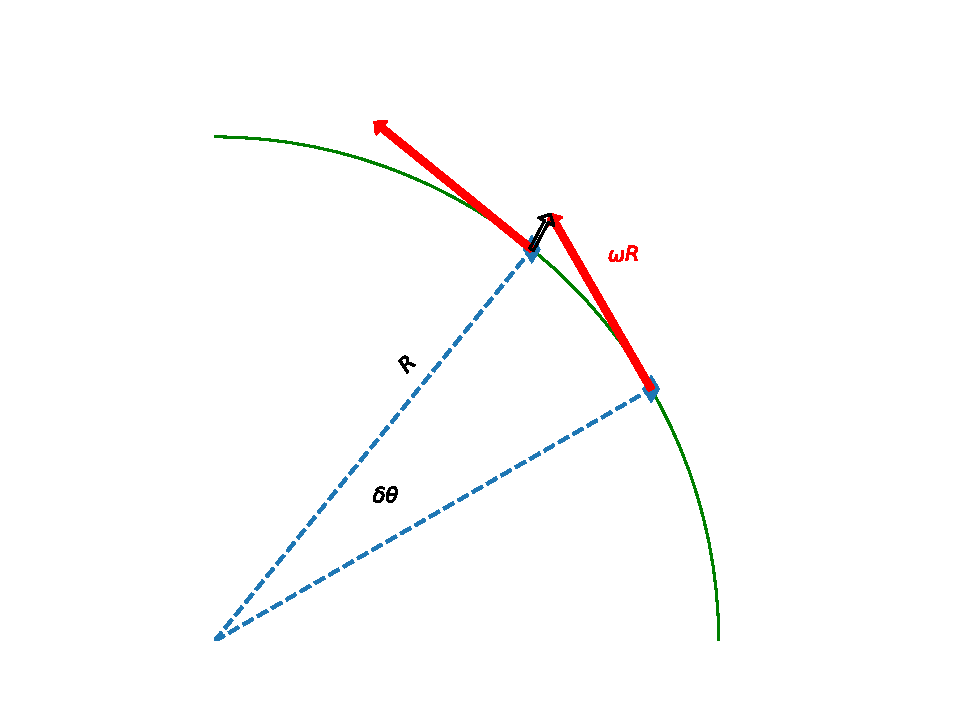
\includegraphics[width=2in]{figs/Waves/CentrifugalForce}
  
Deriving the acceleration  is relatively straight forward.  The angle difference between the two velocity vectors is $\delta \theta$, so the velcoity difference is $\delta v = \omega R \sin(\delta \theta)$, and if $\delta \theta$ is small $\delta v \approx \omega R\, \delta \theta$, or dividing by the time it took to traverse the small change in angle, $\delta t$: $a_c = \omega R \,\delta\theta/\delta t = \omega^2 R$, with the direction away from the axis of rotation.  
\end{derivbox}

\section{The reason for various tidal frequencies}

The various frequencies observed in the tides arise naturally from the net tidal forces (i.e. the tidal bulges) caused by the moon and the sun.  Understanding their origin requires remembering some basic things about the orbit of the moon around the earth and the earth around the sun.  But a few things to keep in mind are
\begin{itemize}
  \item orbital planes are not along the earth's equator, so the tidal bulges are not usually centered at the equator; as we will see below this causes a once-a-day modulation of the tides.  
  \item orbits are not perfect circles, but rather ellipses, so there are modulations if the earth is closer or further away from the sun or moon. 
\end{itemize}

\subsection{Twice a day tides}

\paragraph{$M_2 = 12.42 \mathrm{h}$: lunar semi-diurnal} The tidal bulge made between the moon and the earth means that as the earth spins on its axis, a given point on the earth passes through two high points in the bulge and two low points in the bulge every time that point catches up the to the moon (\fref{fig:AboveEq}. Because the earth and the moon rotate in the same direction, this means that the moon has done 1/29.53 of its orbit in one 24 h period, and hence the bulge has rotated.  The time it takes for the earth to catch up with the moon again is given by $t\omega_{E} = t\omega_M + 2\pi$ or in terms of the periods: 
\begin{equation}
  t = \frac{T_M T_E}{T_M - T_E} = 24.84\ \mathrm{h}
\end{equation}
or a high and low tide every 12.42 h. 

Note that we have used the \Wikiref{synodic month} or \Wikiref{lunar month} of 29.53 days for the period of the moon, despite the fact we said the moon orbits the earth every 27.3 days.  The moon actually does travel 360 degrees around the earth in 27.3 days, but the earth moves relative to the sun, so the moon has to orbit further to be at the same orientation of the earth and sun, and this takes 29.53 days; for a nice animation see \href{http://www.sumanasinc.com/webcontent/animations/content/sidereal.html}{here}. Note that this is derived with the same equation as above with $T_M = 27.321 \ \mathrm{d}$, and $T_S=365.256\ \mathrm{d}$, to yield a period of 29.53 days.  

\begin{figure}[hbtp]
  \begin{center}
    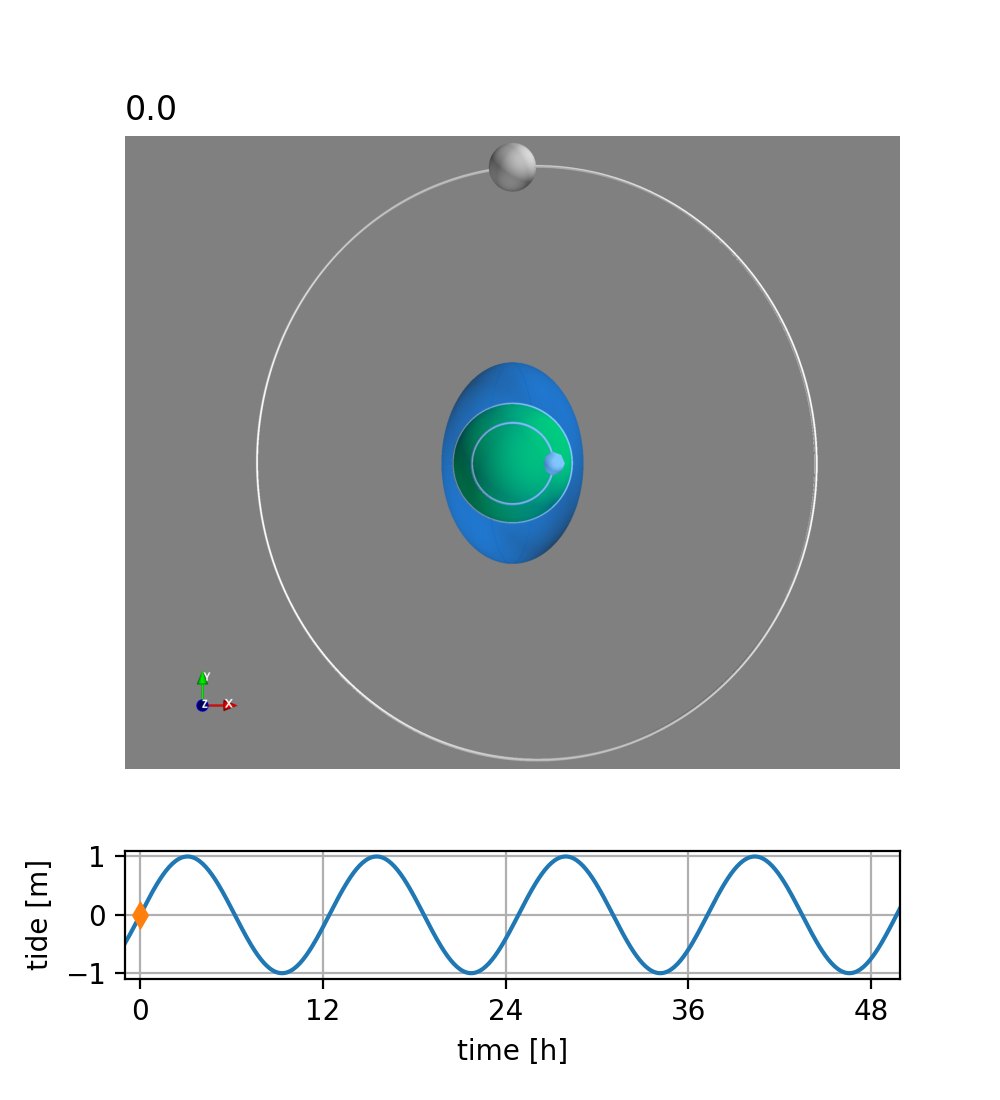
\includegraphics[width=1.75in]{figs/Waves/AboveEq/frame0000}
    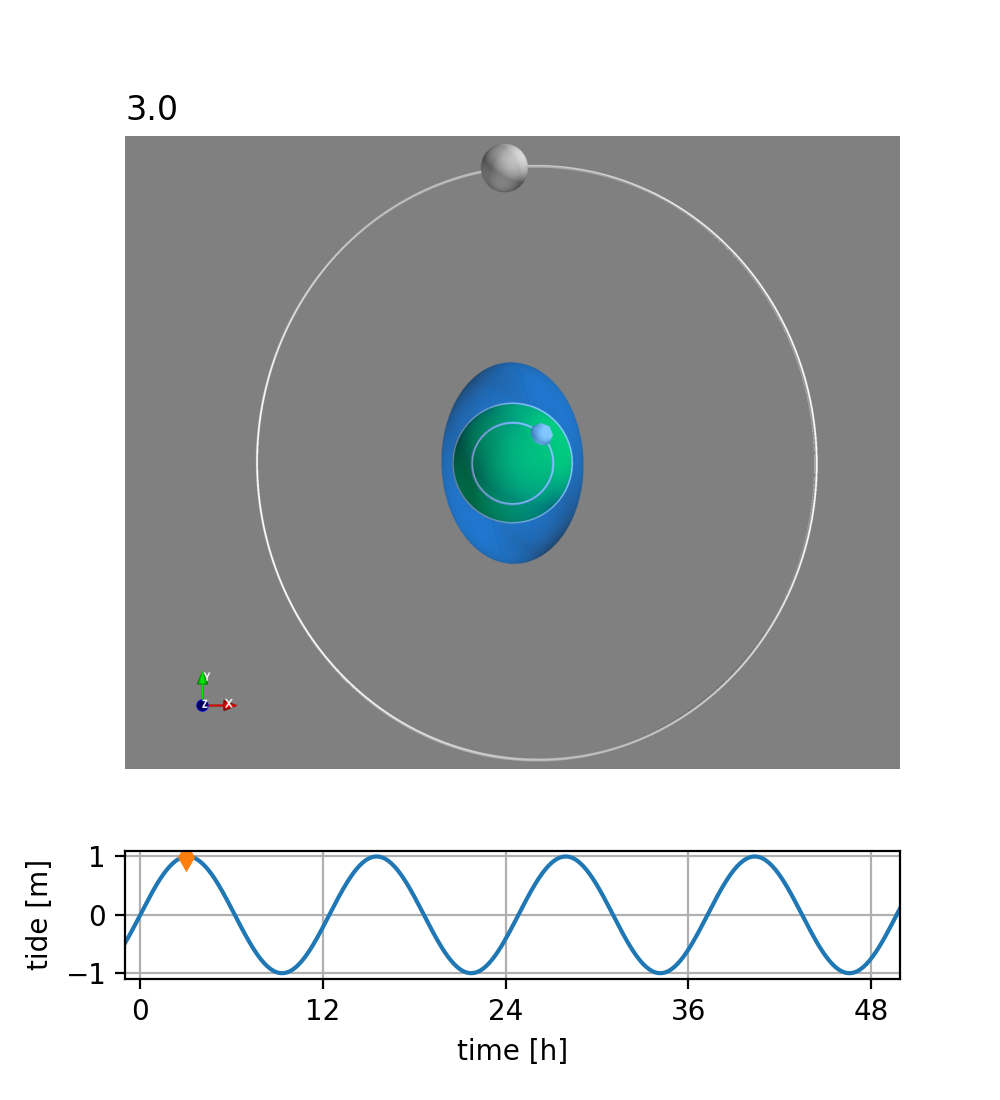
\includegraphics[width=1.75in]{figs/Waves/AboveEq/frame0030}
    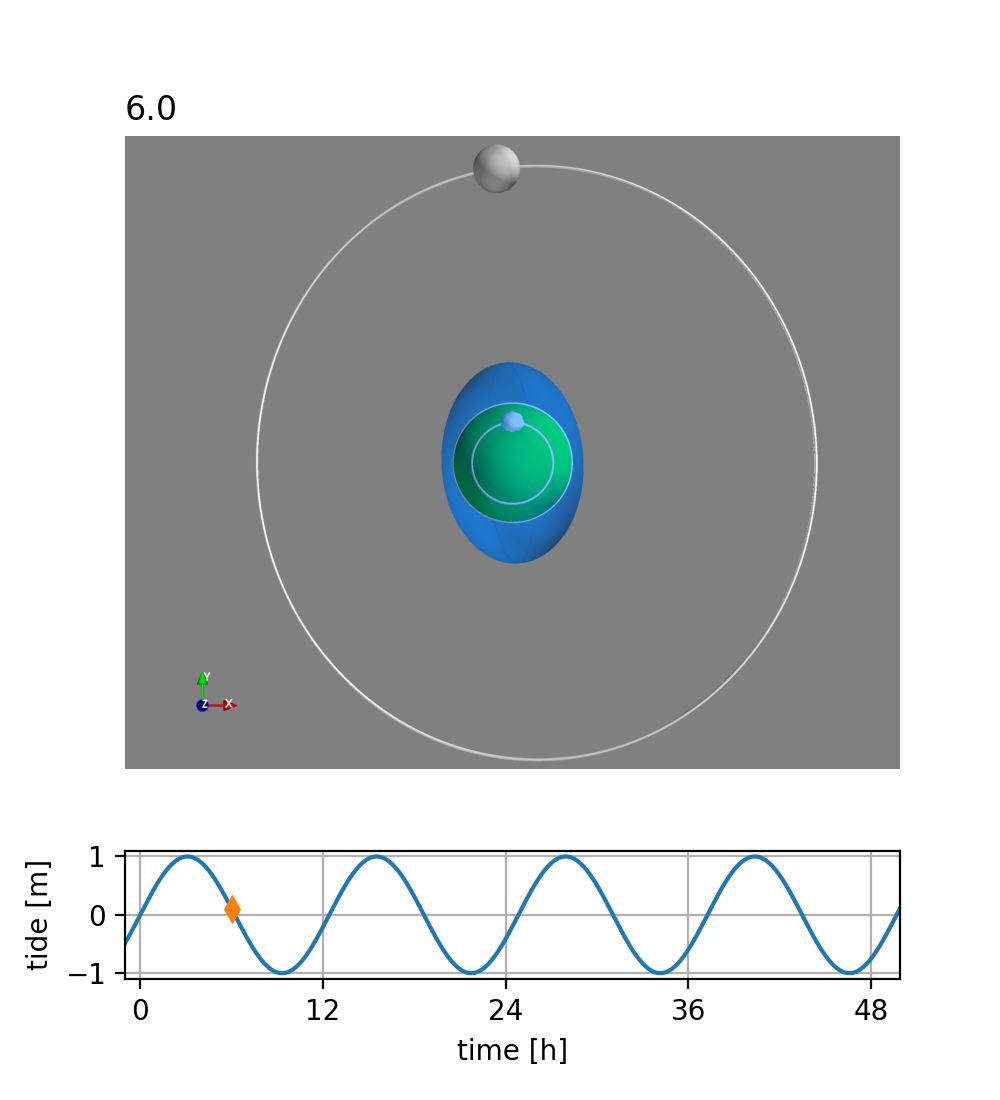
\includegraphics[width=1.75in]{figs/Waves/AboveEq/frame0060}
    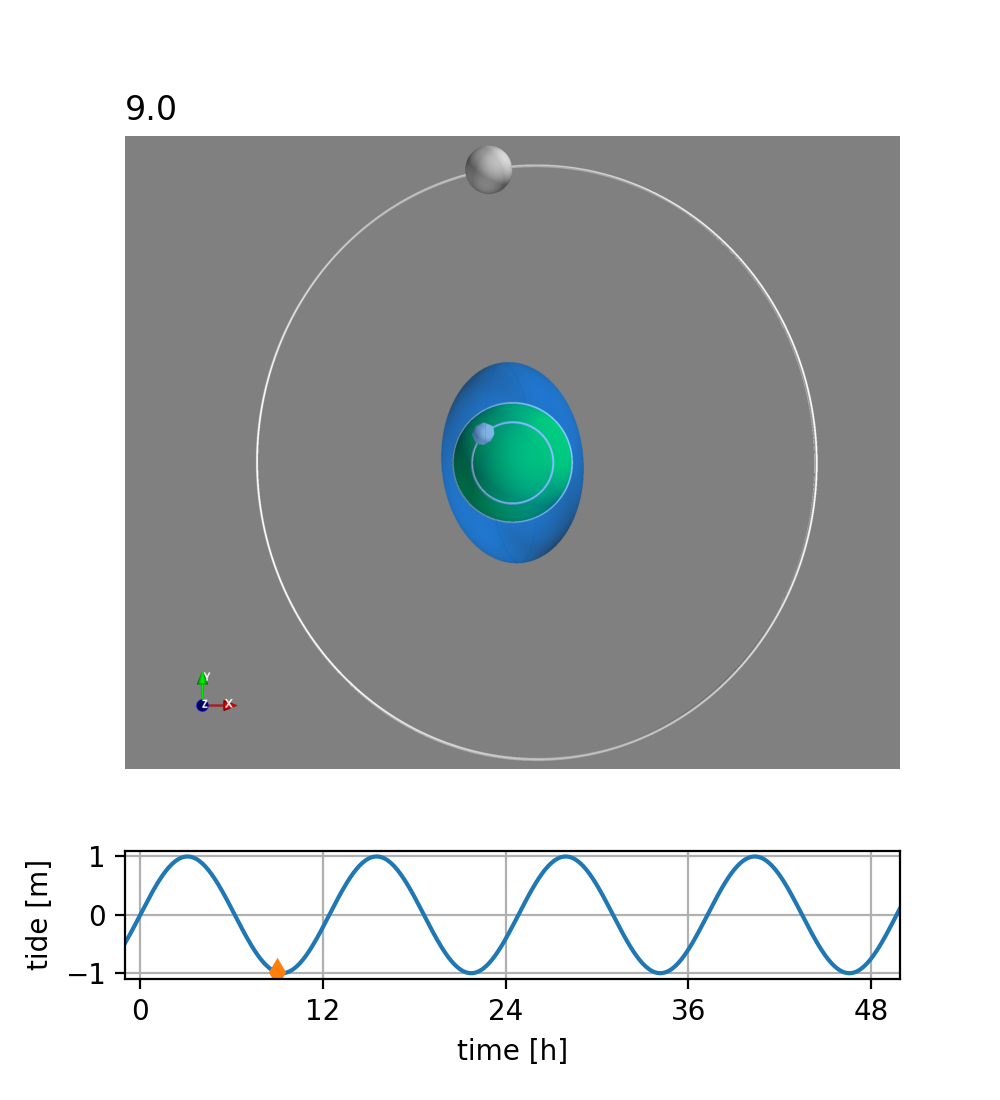
\includegraphics[width=1.75in]{figs/Waves/AboveEq/frame0090}
    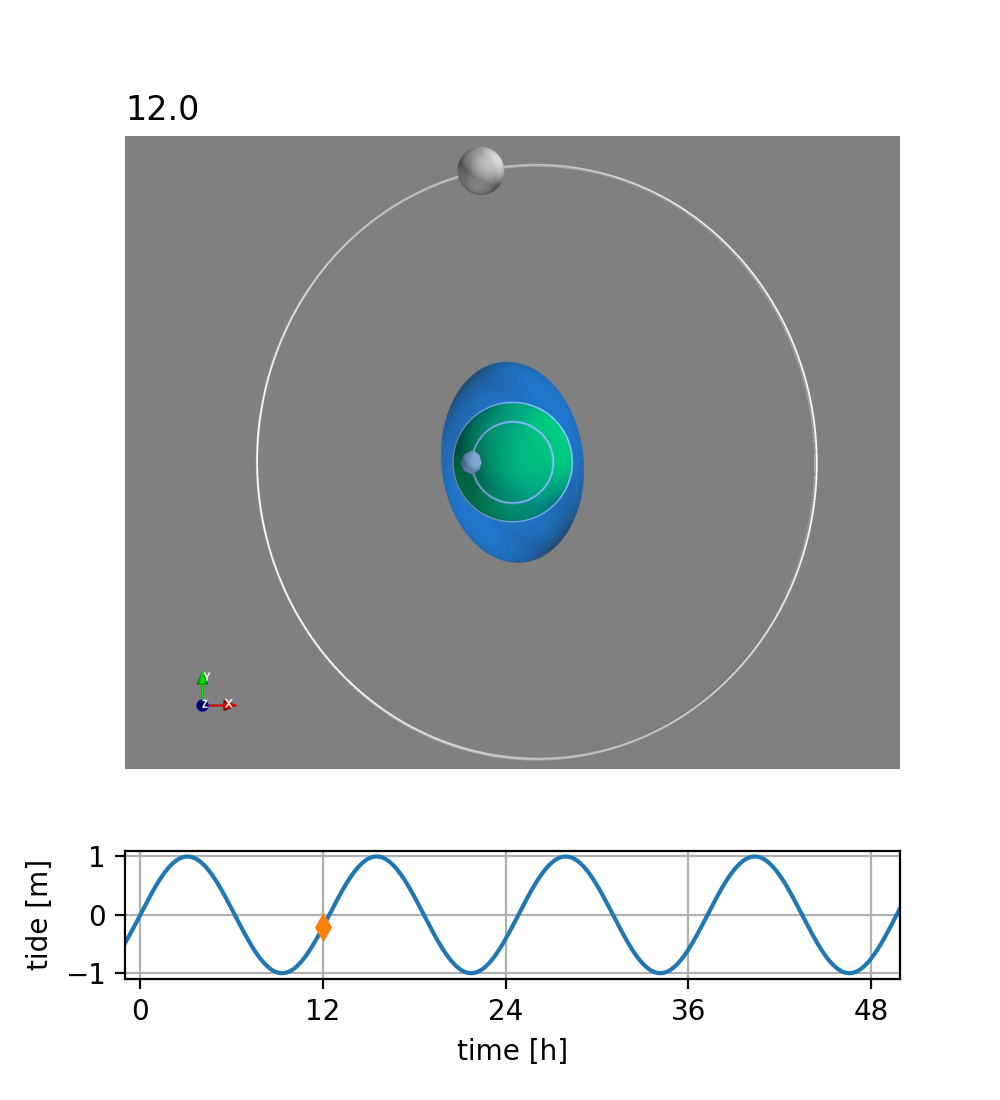
\includegraphics[width=1.75in]{figs/Waves/AboveEq/frame0120}
    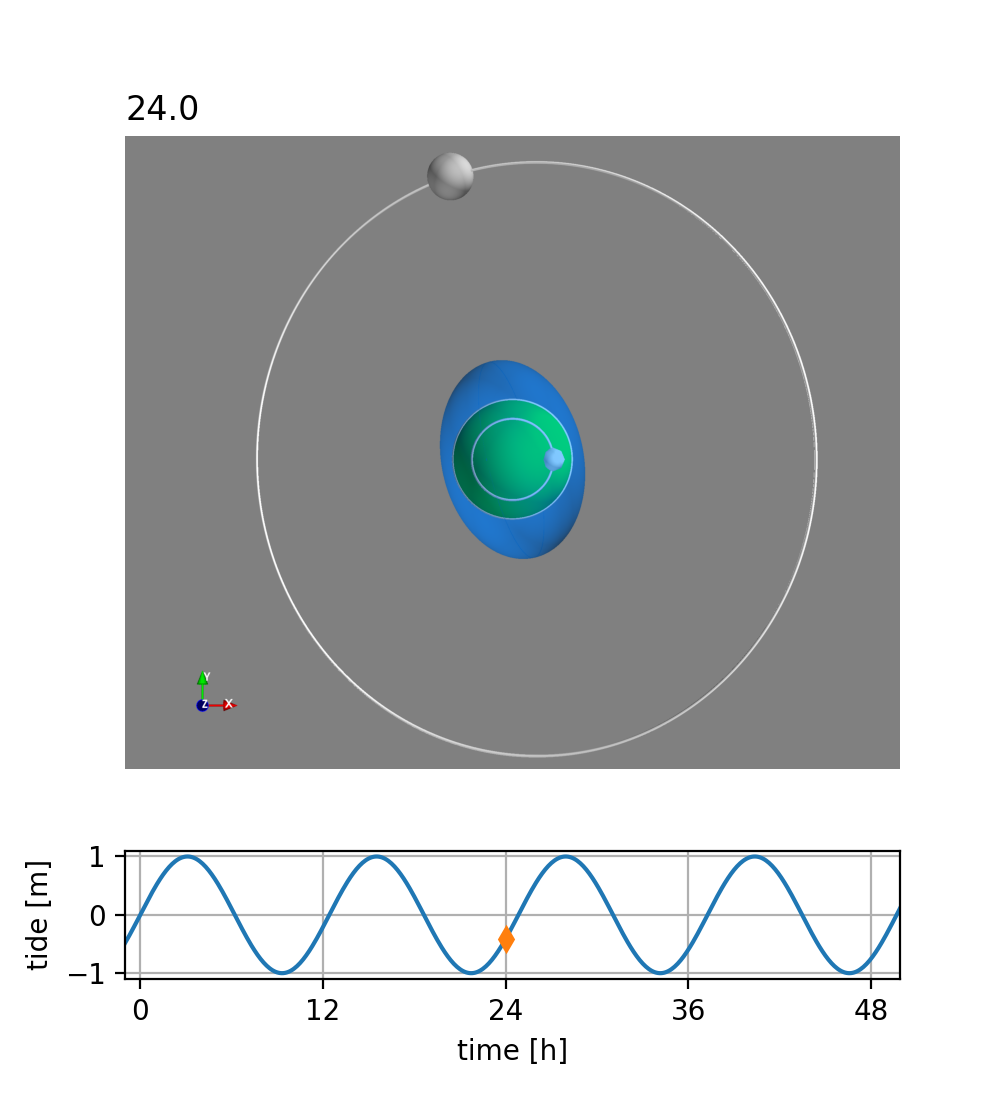
\includegraphics[width=1.75in]{figs/Waves/AboveEq/frame0240}
    \caption{Origin of twice-a day tides from the moon. Looking at North pole, moon moves counter clockwise.  Earth also spins counter-clockwise. }
    \label{fig:AboveEq}
  \end{center}
\end{figure}

\paragraph{$S_2 = 12\ \mathrm{h}$; solar semi-diurnal: spring-neap cycle}
In exactly the same way as the moon, the sun creates a tidal bulge, and this leads to a 12-h tide as the earth turns to face the sun every 24 h, leading to the $S_2$ tide.  The strength of the $S_2$ tide is generally weaker than the $M_2$ tide, because the moon is closer, even though much less massive than the sun.  The relative strengths vary, depending on the time of month, time of year, etc, but we saw above in \fref{tab:TideConst} that $S_2$ was less than 1/3rd $M_2$; globally they average out to be about half the lunar tide.  

Nonetheless, the interference of $S_2$ and $M_2$ create a modulation to the $M_2$ tides that we call the \emph{spring-neap} cycle to the semi-diurnal tide.  As the moon orbits the earth, the tidal bulge moves with it, but the tidal bulge due to the sun only moves slowly as the earth orbits the sun, and the moon and sun's tidal effects are in quadrature ever half lunar synodic orbit (29.53/2 = 14.77 days).  
 
\begin{figure}[hbt]
  \begin{center}
    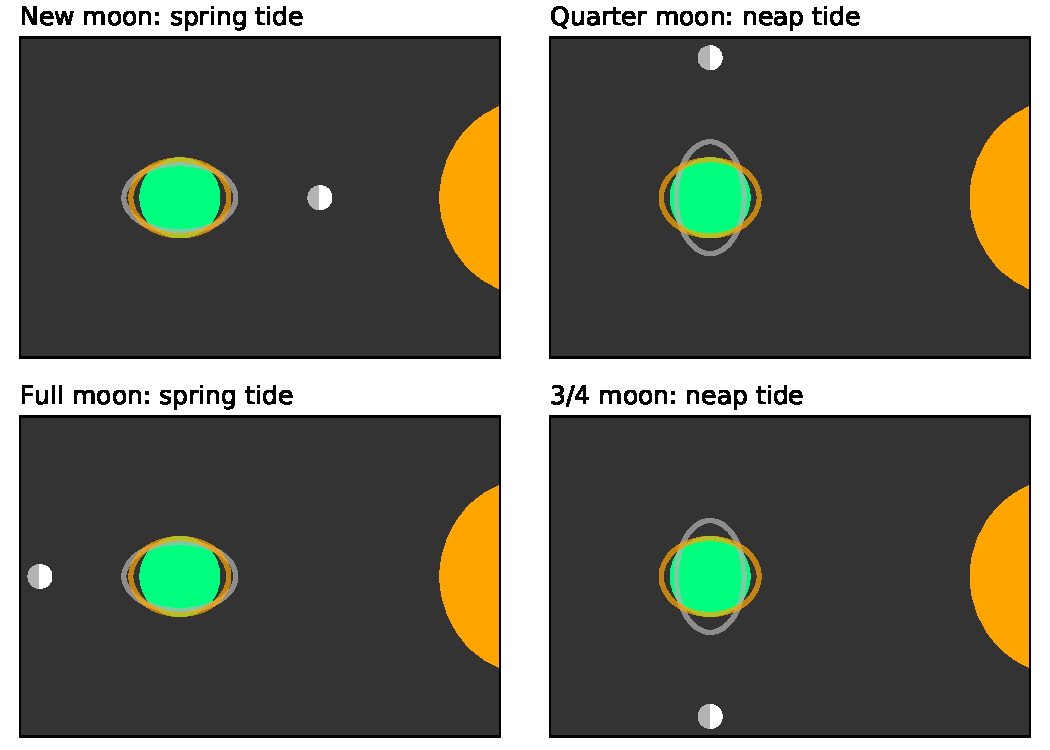
\includegraphics{figs/Waves/TidalBulges}
    \caption{}
    \label{fig:Schematic of tidal bulges due to moon and sun during the four phases of the moon. When the bulges line up (new and full moon) there is a spring tide, and when they are at 90 degrees it is a neap tide.  A new moon occurs ever 29.53 days.  }  
  \end{center}
\end{figure}

Mathematically, we can see that adding an $S_2$ and $M_2$ tide gives us a modulation with a period of  $S_2 M_2 / (M_2 - S_2) = 14.75\ \mathrm{days}$, which is the half the synodic orbit  (the one relative to the su, which we have to line up with) period of the moon (\fref{fig:M2S2}).  

\begin{marginfigure}
    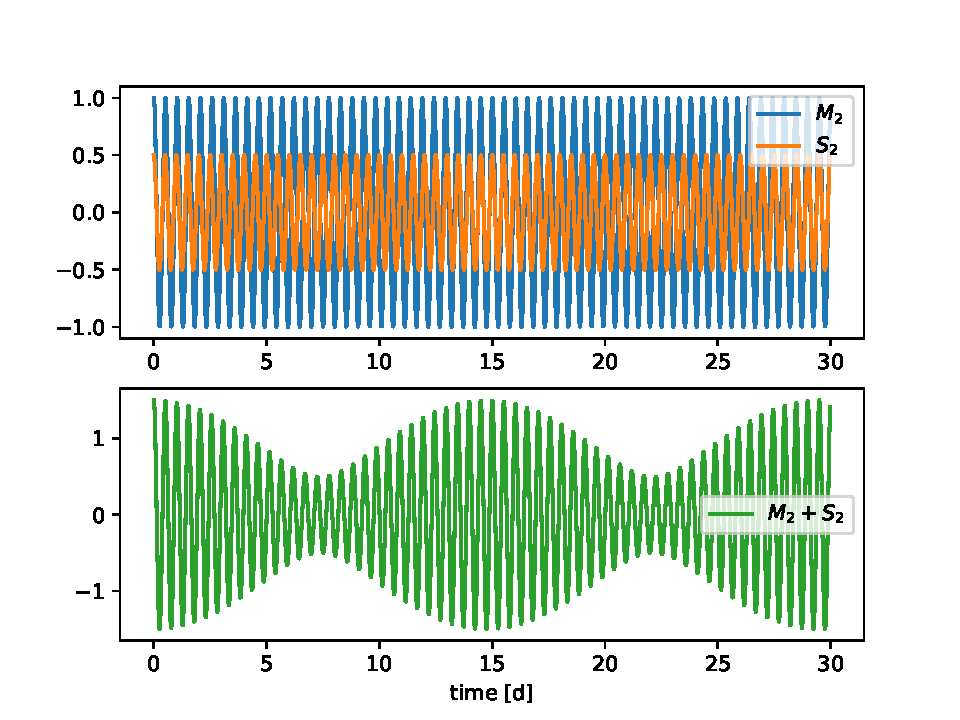
\includegraphics[width=2.7in]{figs/Waves/M2S2}
    \caption{Adding an $M_2$ and $S_2$ wave together, giving a spring-neap cycle that repeats every 14.77 days.}
    \label{fig:M2S2}
\end{marginfigure}

\subsection{Daily tides (diurnal): Tides due to non-equatorial orbits}

The moon's orbit is not along earths equator, and the earth is tilted relative to the sun.  So the tidal bulges that these bodies cause are not centered on the equator, but rather are tilted.  As the earth spins through these bulges, there are still two high tides, but one of them will be larger than the other, adding a \Wikiref{diurnal} component to the tides.  

\paragraph{Moon's declination} The \Wikiref{moon's orbit} is at an angle to the equator.  Currently that angle is about 21 degrees, but it varies between 18 and 28 degrees on a 18.6-year time scale (\fref{fig:Lunar-Declination}).  This precession of the moon's orbit  leads to an 18.6-y cycle in the tides that must be kept track of!

\begin{figure}[hbt]
  \begin{center}
    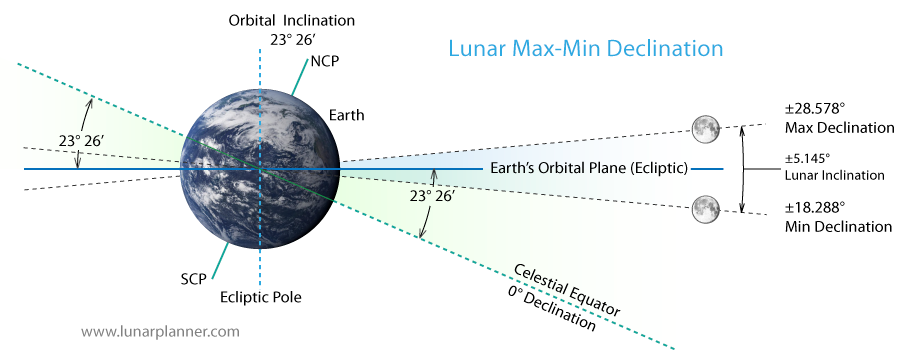
\includegraphics{figs/Waves/Lunar-Declination}
    \caption{Schematic of the lunar declination, and the earth's tilt relative to its orbital plane around the sun.  Note these tilts mean that the tidal bulges are not symmetric about the earth's equator.}
    \label{fig:Lunar-Declination}  
  \end{center}
\end{figure}

The result of this title relative to the equator means that the tidal bulge is also inclined between 18 and 28 degrees from the equator.  As a point on the norther hemisphere spins through this bulge, there are still two high tides, but one will be larger than the other (\fref{fig:SideLow}).  

\begin{figure}[hbtp]
  \begin{center}
    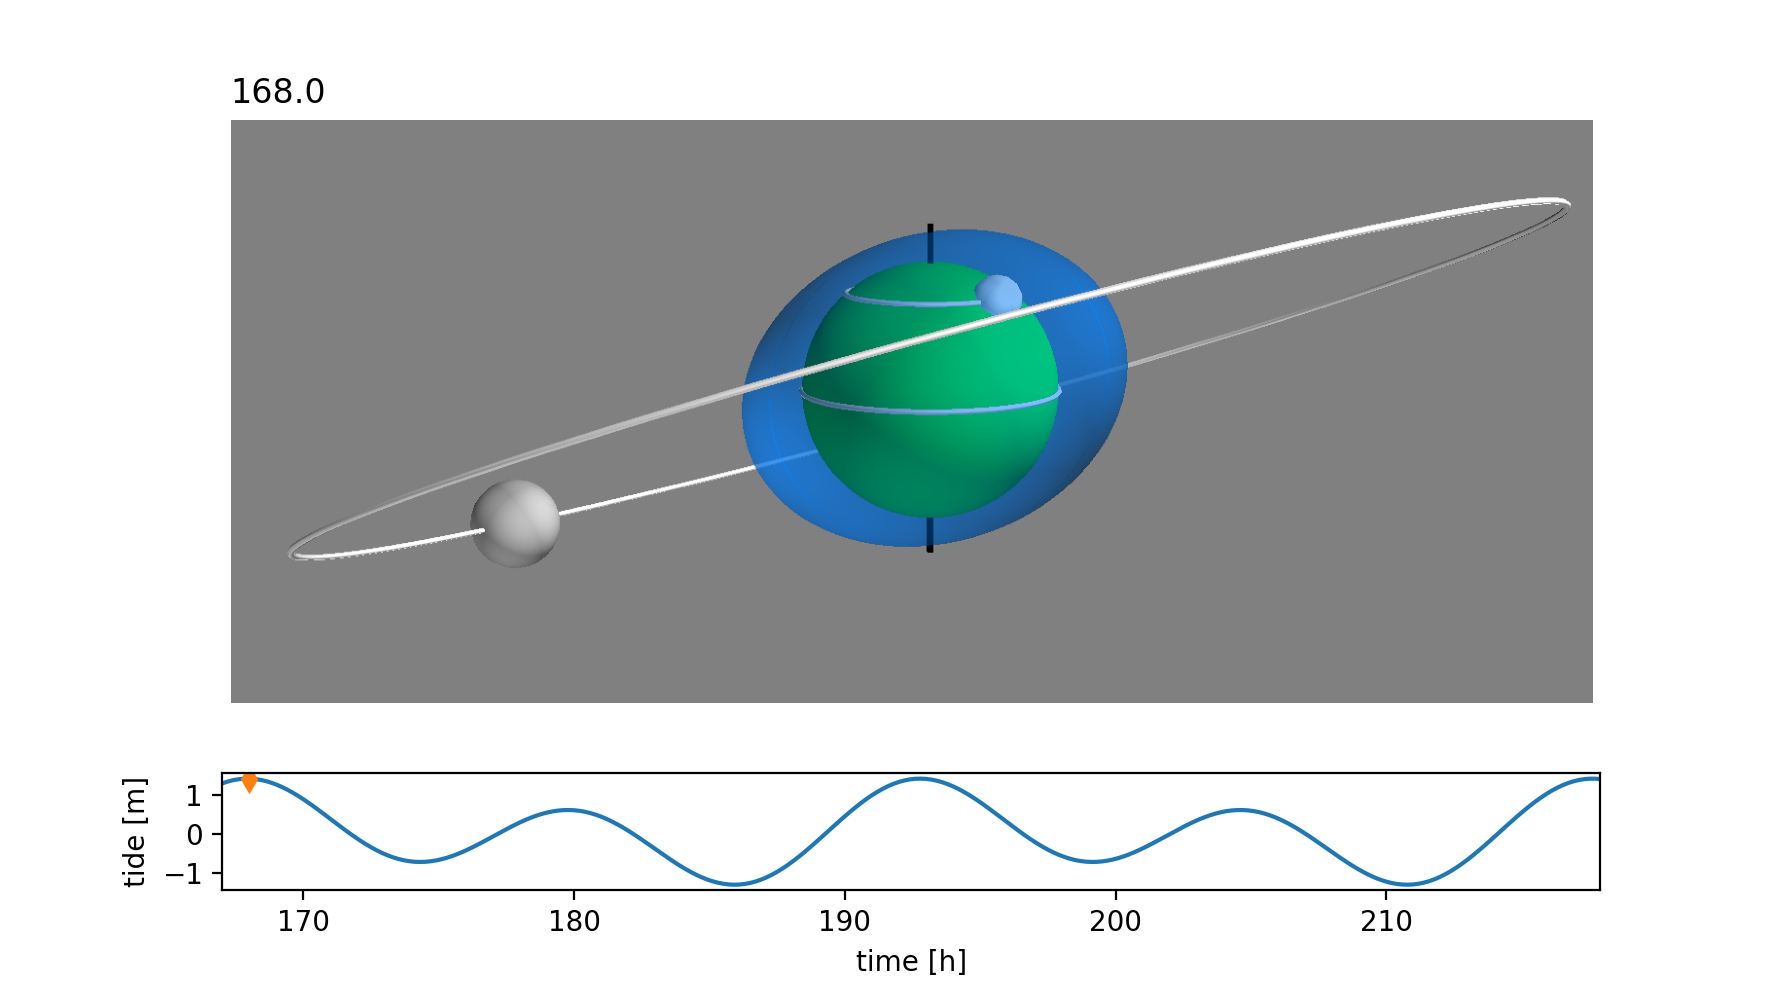
\includegraphics[width=2.1in,trim=40 20 50 20,clip]{figs/Waves/SideLow/frame1680}
    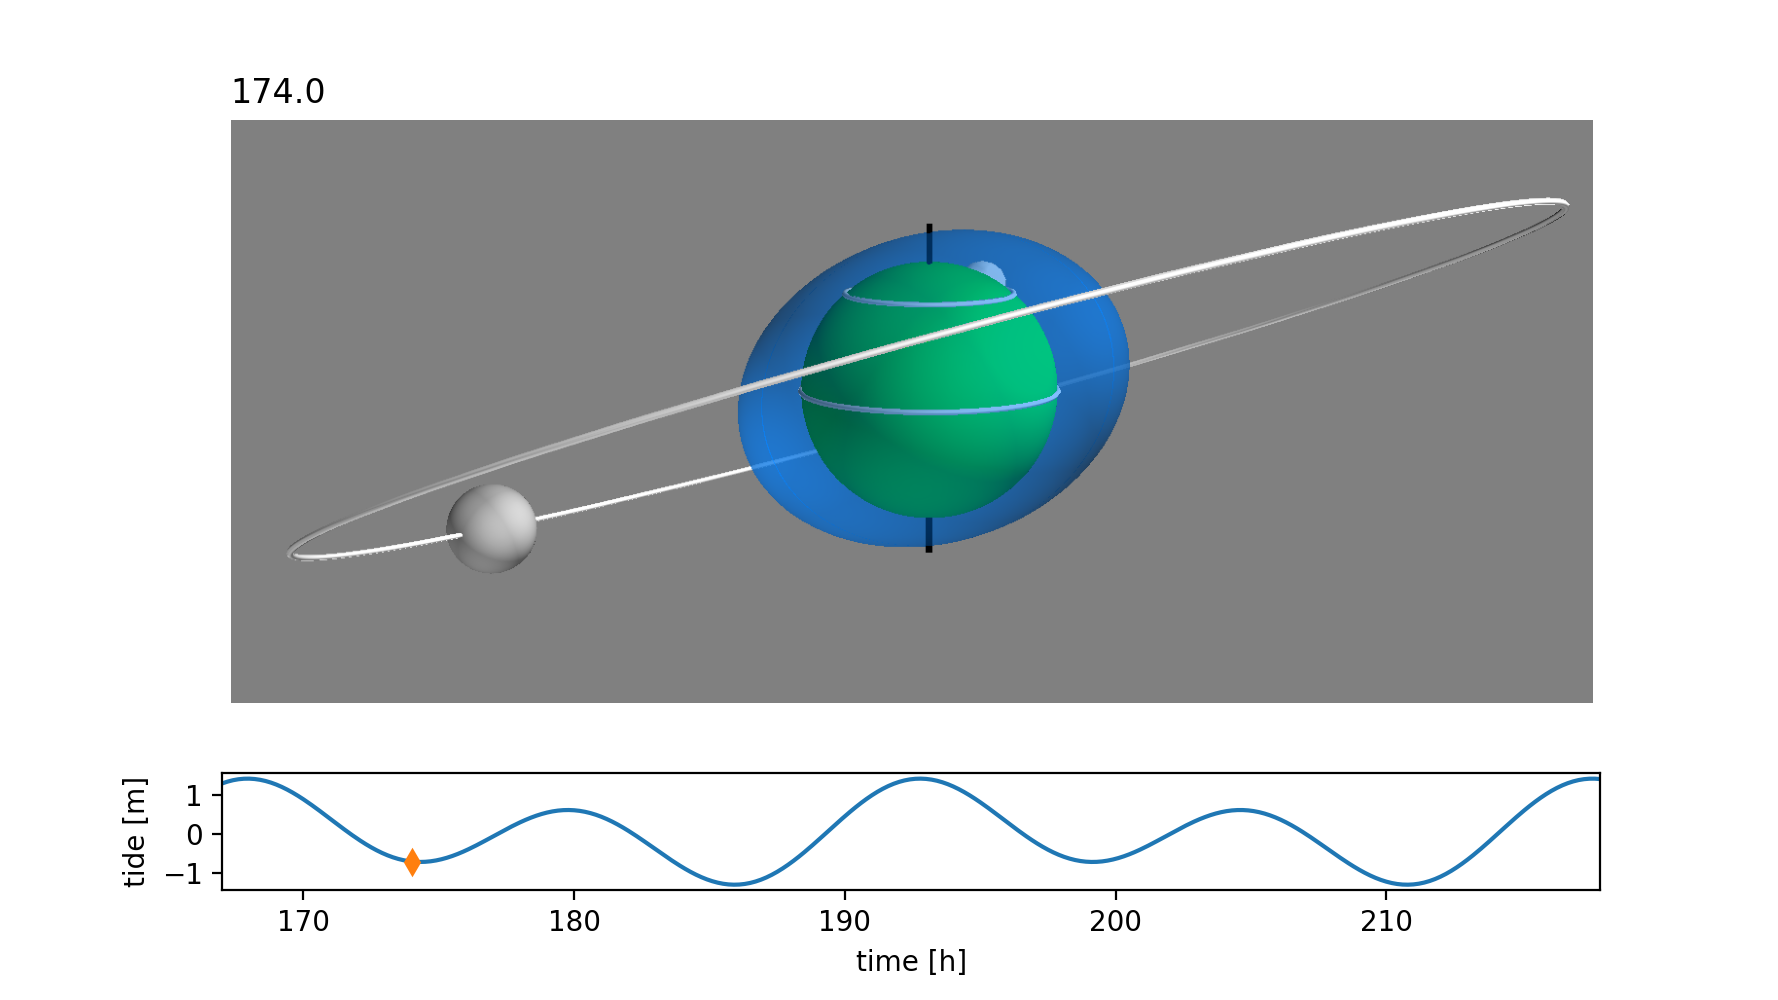
\includegraphics[width=2.1in,trim=40 20 50 20,clip]{figs/Waves/SideLow/frame1740}
    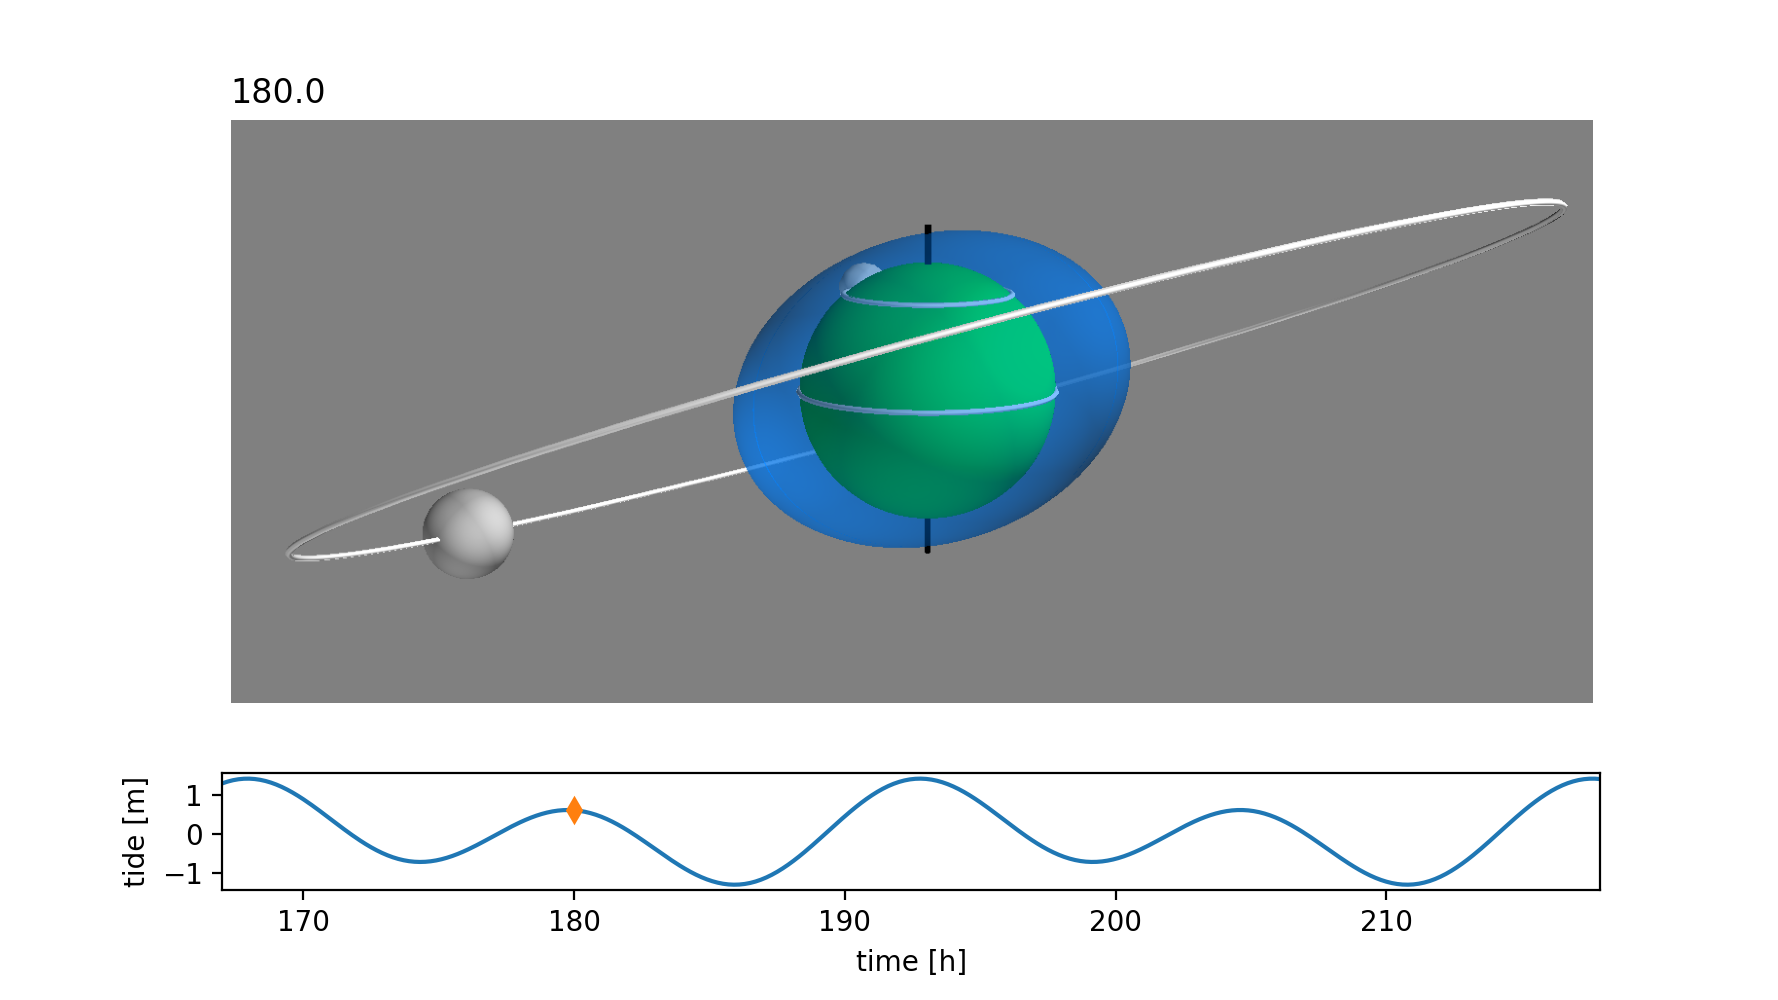
\includegraphics[width=2.1in,trim=40 20 50 20,clip]{figs/Waves/SideLow/frame1800}
    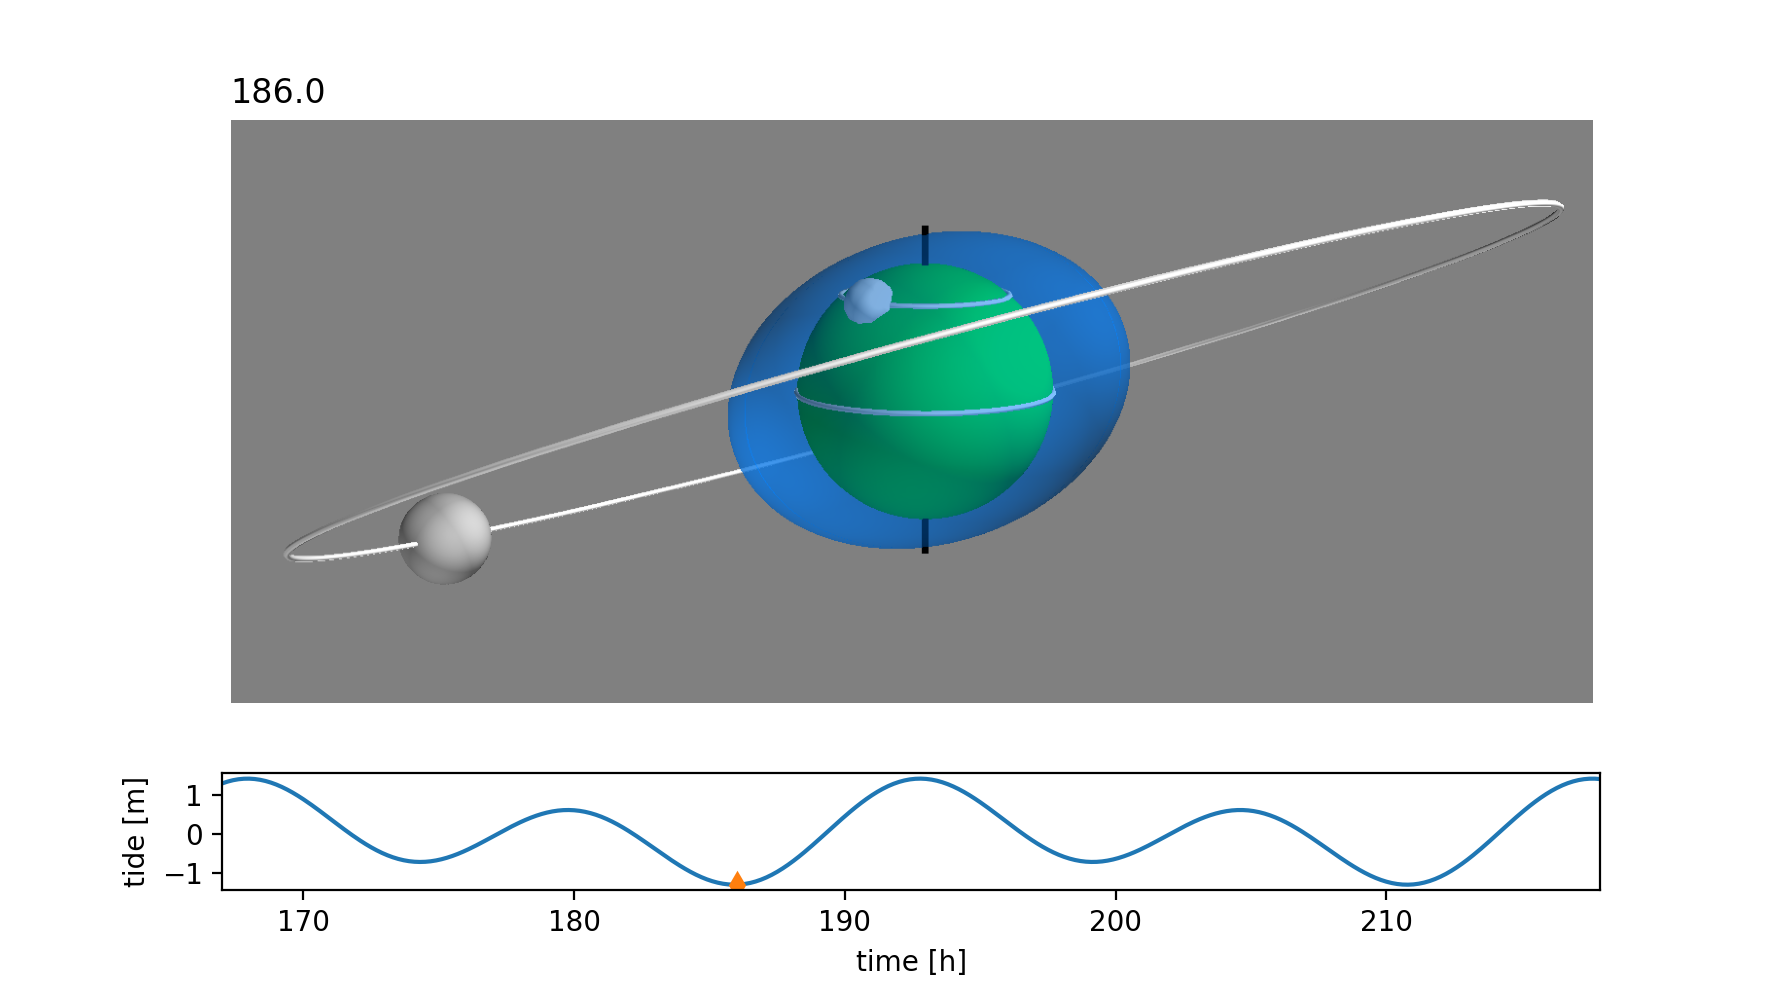
\includegraphics[width=2.1in,trim=40 20 50 20,clip]{figs/Waves/SideLow/frame1860}
    \caption{Origin of once-a-day tides from the moon. Here the moon is at the point of its orbit when it is 20 degrees below the equator.  So the tidal bulge is large on the northern hemisphere away from the moon.  An observer on the northern hemisphere sees a larger high tide when pointed away from the moon, and a lower high tide on the side nearest the moon. }
    \label{fig:SideLow}
  \end{center}
\end{figure}

Mathematically, we represent this as a daily modulation on the twice-a-day tide by adding a ``diurnal'' component to the tide (\fref{fig:M2K1}).  This has the obvious effect of making the high tide higher once every two high tides.  Note also that there is an assymetry to the high-high and low-low tides just from these two components that make the high-highs larger ever two weeks, and the low-lows larger on opposite weeks.  Note, however, that this does \emph{not} happen with the real moon, because the real moon changes its angle throughout the orbit of the moon, and the strength of the $K_1$ diurnal component is modulated by the $O_1$.  Note that the $K_1$ and $O_1$ tides create a 13.66 day beat, which is half of the \emph{sidereal} (or from space, versus relative to the sun) orbit period of the moon of 27.3 days.  
 
 \begin{figure}[hbt]
  \begin{center}
    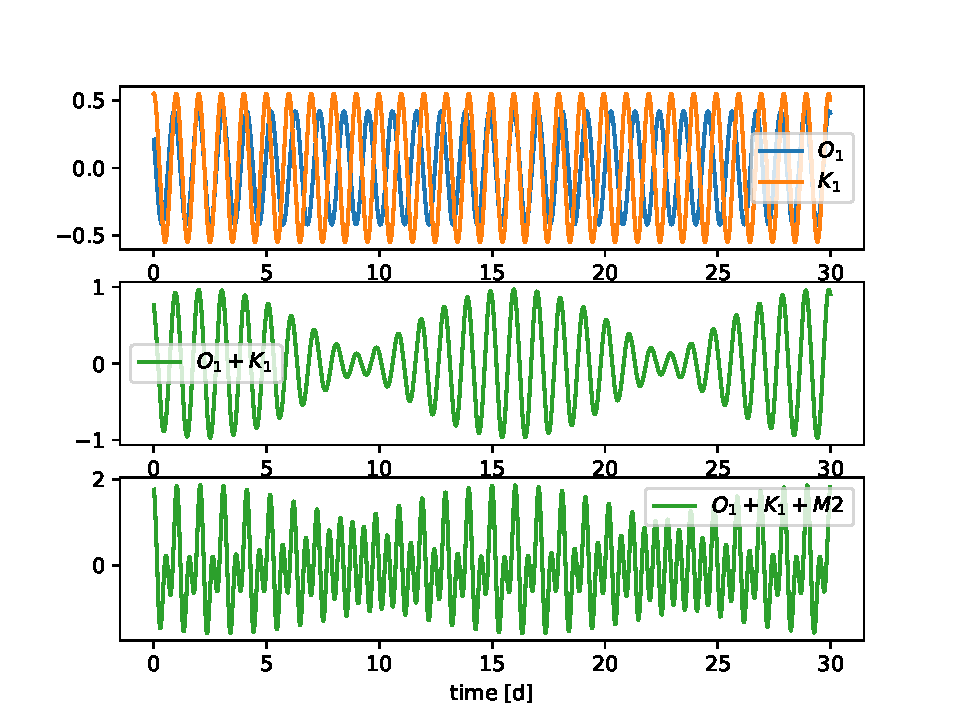
\includegraphics{figs/Waves/M2K1}
    \caption{Adding a diurnal frequency tide to a semi-diurnal that varies in strength every two weeks. $K_1=23.934 \ \mathrm{h}$ and $O_1 = 25.819\ \mathrm{h}$ are lunar-diurnal tides and added together they are modulated every 13.66 days}
    \label{fig:M2K1}  
  \end{center}
\end{figure}

\paragraph{Solar declination} Similarly, the earth is inclined towards the sun, with the northern hemisphere tilted 23.43 degrees towards the sun in the northern hemisphere summer solstice.  This similarly causes an asymmetry in the solar tidal bulge, and a diurnal component to the solar tides.  These have a similar character to the changes due to the moon's declination, however, their strength varies through the \emph{year} rather than through the lunar month.  The solar diurnal component pair are $S_1=24\ \mathrm{h}$ and $P_1=24.06588766\ \mathrm{h}$, and the beat between them is one year.  

\subsection{Longer period tides}  Finally, there is a weak dependence of the tide on how close the moon is and how close the earth is to the sun.  When the moon is closes to the earth it is called \Wikiref{perigee}, and the opposite is \Wikiref{apogee}.  The perigee is about 10\% of the moon's mean orbit of about 400,000 km , so this has a significant effect on the tides.  The perigee and apogee precess with time, so they are not tied to the declination, and have a period of 27.554 days.  This precession has a period of about 4 years.  

The equivalent frequency is an annual change in the earth's distance from the sun, or perihelion and aphelion.  The difference is about 2.5 million km out of 149.5 million km, so a much less pronounced of an ellipse than the lunar orbit.  Currently, perihelion occurs the first week of January (5 January for 2020) and aphelion the first week of July (4 July, 2020).    That it occurs near the solstices is a co-incidence, though, and the ellipticity of the earth's orbit around the sun varies on a time scale of 22,000-26,000 years.  

As noted above the declination of the moon varies on an 18.6 year time scale  between 18 and 28 degrees with respect to the equator, so we expect lunar diurnal tides to vary on this time scale as well.  The importance of this is hard to see, but there is evidence that this change in tides affects the strength of ocean mixing, particularly in straits that have strong diurnal tides, and that this can have a noticeable affect on ocean temperature \citep{mckinnellcrawford07}, and oxygen levels \citep{crawfordpena16}, possibly due to mixing in the Sea of Okhotsk \citep{yasudaetal06}.

Finally, the tilt of the earth varies with a period of about 41,000 y.  These variations are thought to have only been between 22 and 24 degrees, but are thought to have long-timescale climatic effects, called \Wikiref{Milankovitch cycles}.  

\section{Dynamic theory of the tides}

If a real tidal bulge were to travel around the earth, it would need to travel 40,000 km around the equator in 24 h, or travel at a speed of 465 m/s.  Assuming this is a shallow water wave, the ocean would have to be 22km deep.  Further, of course, the ocean would have to be continuous, with no land masses blocking the progress of the wave.  Therefore, instead we should think of the tidal bulge as a forcing that the ocean responds to.  The details of that response depend on the shape of basin, and sources of loss from the surface tide to other smaller scale processes (e.g.\ friction, making internal tides, etc).  

\subsection{Tidal Resonance}

The most obvious example of the tidal response depending on the shape of the basin is to think about what happens in a fjord.  Consider a fjord that is approximated as a long rectangular basin, say $H=200\ \mathrm{m}$ deep,   with a mouth into a much deeper and larger ocean.  The tidal forces act on the small fjord, but are completely swamped by the tides that the mouth of the fjord sees.  So this is a situation where the body doesn't even notice the astronomical forcing by the tides, let alone be driven by them.  Similarly, the ocean barely notices the presence of the fjord, and the tides in the ocean can ignore the motions in the fjord. 

In this idealization, we can prescribe the forcing at the mouth of the fjord in terms of a sea level change that is a sine wave in time, e.g. $\eta(x=L, t) = \eta_0 \sin(\omega t)$ (\fref{fig:SketchFjord}).  The \emph{response} of the fjord is simply a pair of waves, one propagating into the fjord, and one reflecting.  Because no energy is lost, both waves have the \emph{same} amplitude, but can have different phases:
\begin{equation}
    \eta = A \sin(\omega t - k x + \phi_{in}) + A \sin(\omega t + k x +\phi_{out})
\end{equation}  
where $\omega/k = \sqrt{gH}$ because the tidal waves are examples of shallow-water waves.  In order to solve for A and the phases, we need a second boundary condition, this one is at the head of the fjord ($x=0$), where we know that the flow must be zero: $u=0$.  Recall that the speed of a wave is proportional to the derivative of the seasurface height, so we can rewrite this as $\frac{d\eta}{dx} = 0$.  Using both these conditions and our doubel angle identities, we can write the solution as:
\begin{equation}
    \eta = \frac{\eta_0}{ \cos kL}\ \sin \omega t \cos kx
\end{equation}
Hopefully, its readily apparent that this solution satisfies the conditions above at $x=-L$ and $x=0$.  

This solution is a \Wikiref{standing wave}.  Notice that everything in the fjord rises and falls at the same time, so high tide happens everywhere at the same time.  Another way of saying this is that there is no change of phase of the tide in the fjord.  Another feature is that the amplitude of the sea surface height at the head of the fjord is larger than the amplitude at the mouth; the opposite applies to the velocities, which are zero at the head, and largest at the mouth.  

\begin{figure}[hbt]
  \begin{center}
    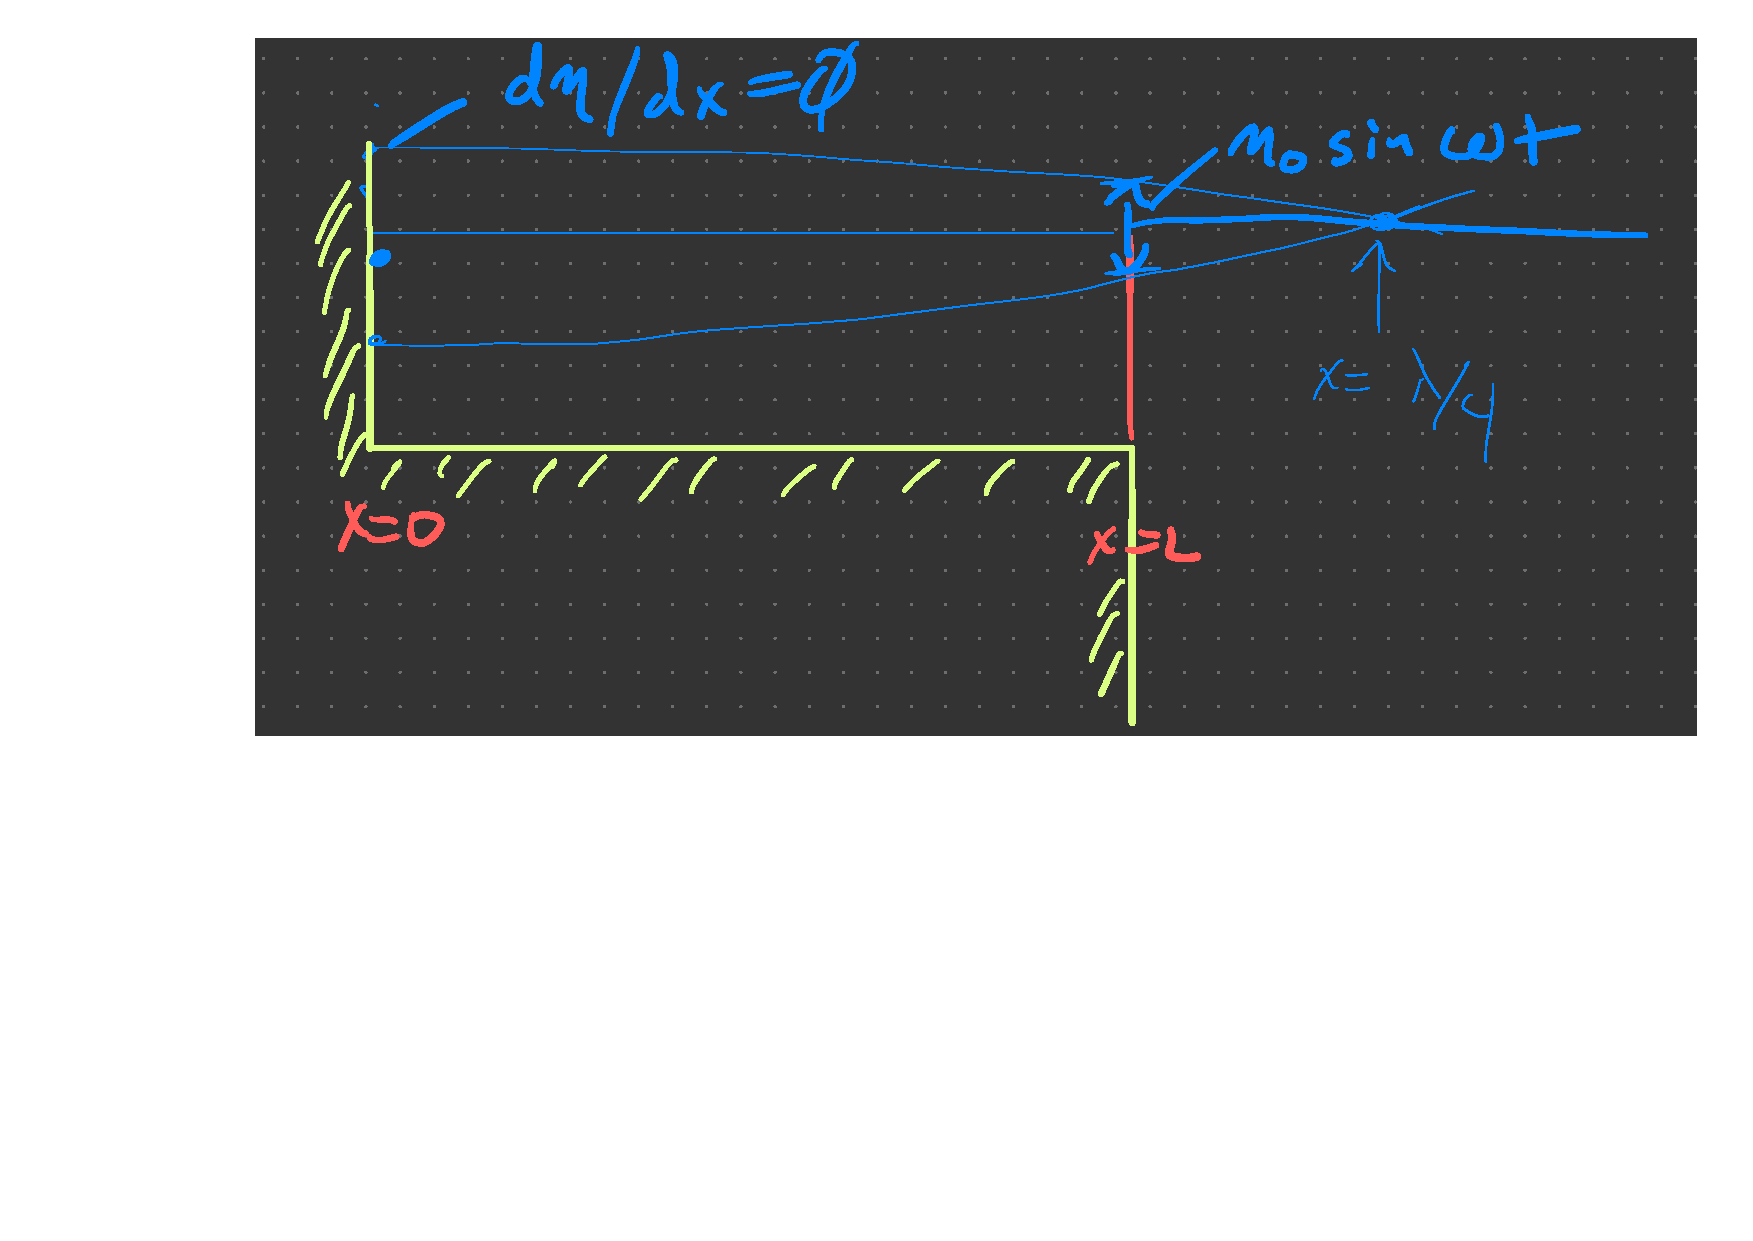
\includegraphics{figs/Waves/SketchFjord}
    \caption{A fjord with a wall at $x=0$ and an ocean at $x=L$.  The wavelength $\lambda=\frac{2\pi}{k}$ is set by the water depth and the frequency of the tide: $k=\frac{\omega}{\sqrt{gH}} $}
    \label{fig:SketchFjord}  
  \end{center}
\end{figure}

The solution depends significantly on the quantity $kL$.  As $kL\to n \pi/2$ the response in the fjord becomes infinite because $\cos kL \to 0$.  This is called \emph{quarter-wave} resonance, and is the same resonance that you get when blowing over a bottle at the right frequency to make a musical note. Any length $L$ fjord with a depth $H$ has \emph{resonant frequencies} given by $\omega = \frac{n\pi}{2L}\sqrt{gH}$, where $n$ is any integer.  A useful way yo think about this is that the response is a sine wave with wavenumber $k$, and if the mouth of the Inlet falls on a "node" of the sine wave, then a resonant response is achieved.  As an example, consider a tide with $T=12.4\ \mathrm{h}$ in a fjord with a water depth of 200 m, then the wavelength of the wave is about 2000 km, and a resonant fjord would have a wavelength of about 500 km (or 1500 km, or 2500 km, etc, but those would be \emph{very} long fjords!).  
 
 Note that as a fjord that is longer than $\lambda/4$ (but shorter than $3\lambda/4$) then the head of the fjord and the moth are 180 degrees out of phase, with the head rising while the mouth sinks.  
 
\subsection{Frictional effects}
 
A frictionless flow is often a reasonable approximation of a deep fjord.  If there is friction, then the reflected wave is weaker than the incoming wave, and the tide will have a \emph{progressive} character with phase changing as the wave propagates into the fjord.  It is possible that the wave is damped completely so that there is no standing component, and the amplitude falls to zero at the head of the fjord.  

\subsection{Global response}

The global response to tidal forcing is quite complex due to the bathymetry and shapes of the ocean basins (\fref{fig:TidalAmplitudes}). In general, the tides create a wave that propagates clockwise around the basin in the northern hemisphere, and counter-clockwise in the southern.  The clockwise circulation (NH) is because of the Coriolis force creating a wave that always has land on its right side (NH).  This can be seen by the increasing value of the phase contoured in \fref{fig:TidalAmplitudes}. The response is such that there are ``nulls'' in the pattern, called \Wikiref{Amphidromic points} where the amplitude of the tide is zero.  Conversely the tides tend to be largest at boundaries of basins.  

\begin{figure}[hbt]
  \begin{center}
    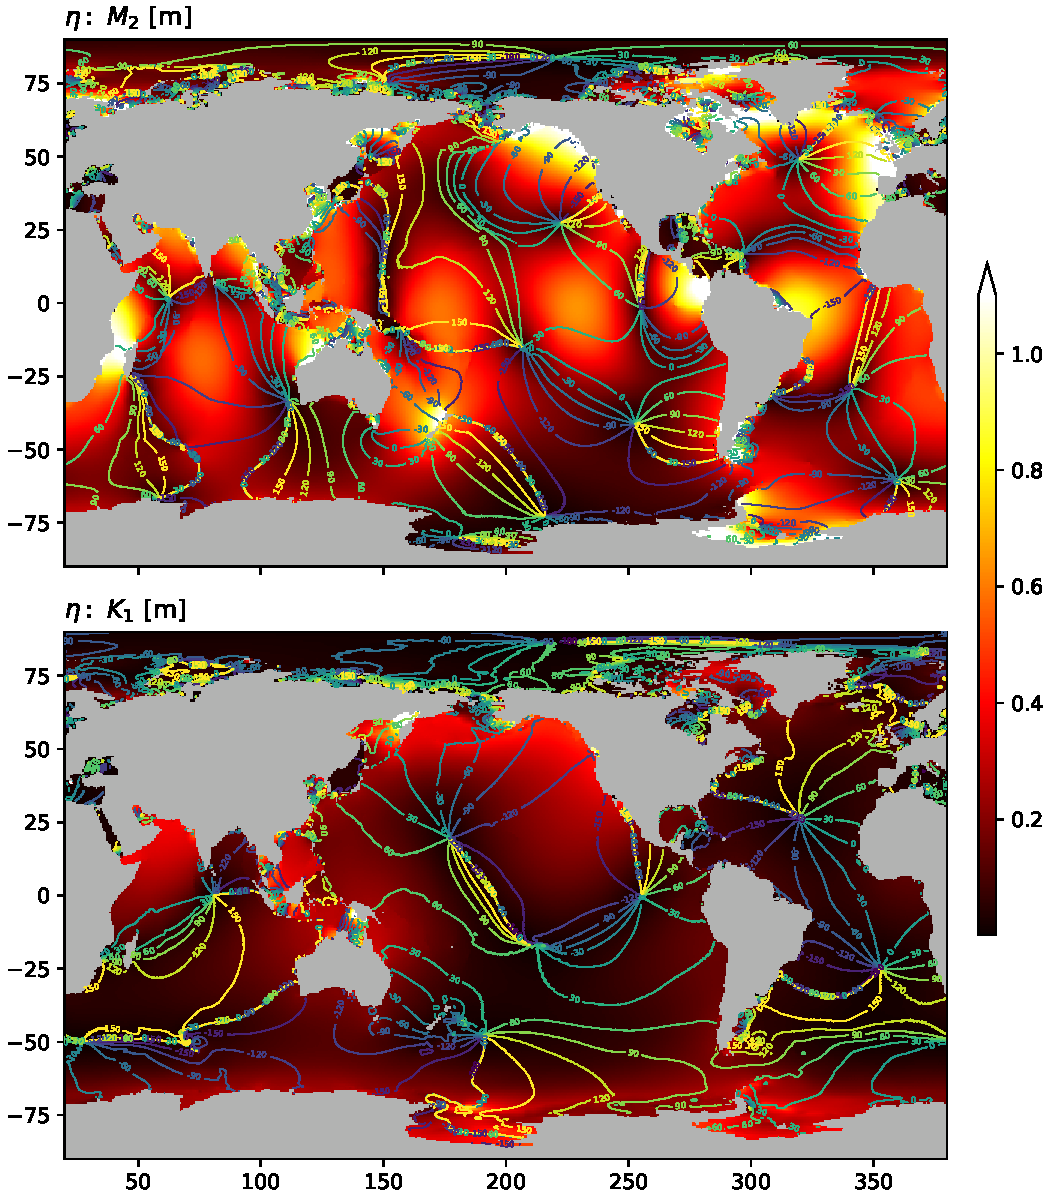
\includegraphics[width=5in]{figs/Waves/TidalAmplitudes}
    \caption{Amplitudes are coloured, and lines of constant phase are contoured in degrees. }
    \label{fig:TidalAmplitudes}  
  \end{center}
\end{figure}

The surface $M_2$ tide in 4000-m of water has a wavelength of $\approx8,800\ \mathrm{km}$, and the $K_1$ tide is $17,000\ \mathrm{km}$, so a wave ``fits'' in the basins very imperfectly.  You can see that, because of its longer wavelength, the $K_1$ tide has fewer amphidromic points than the $M_2$ tide.  
\clearpage

\section{Exercises}

Consider the tidal calendars for Victoria BC, 2020.  Full and new moons are marked (circles), lunar perigee and apogees are marked (P/A), as are the peaks of the moon's declination relative to the equator.  

\begin{center}
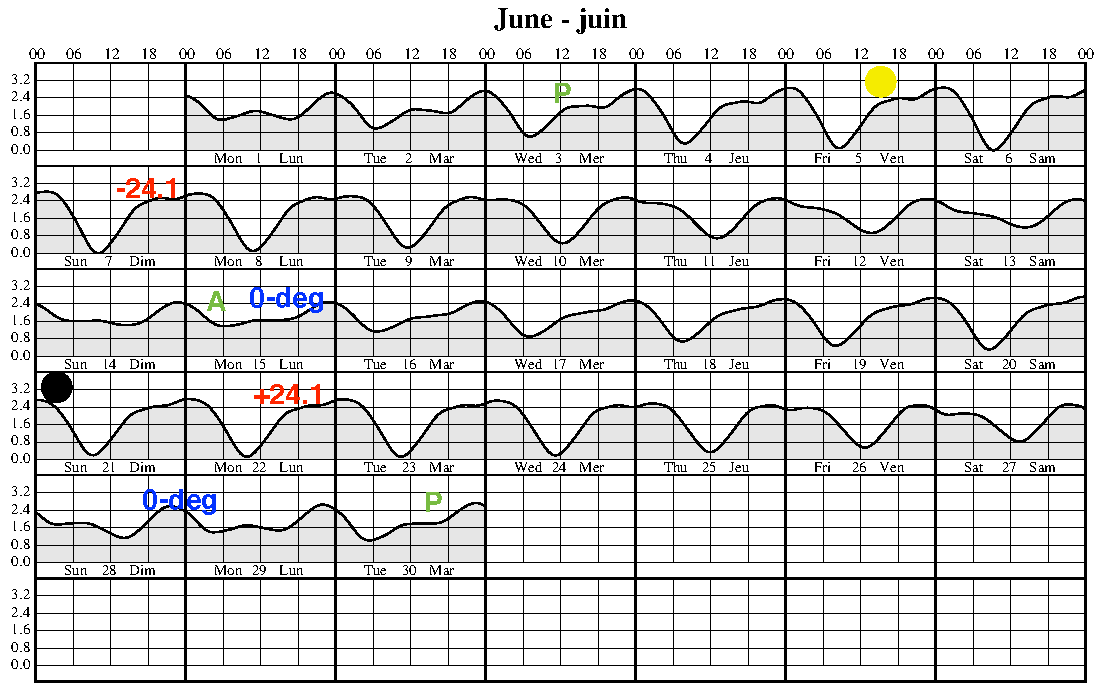
\includegraphics[width=3.7in]{figs/Waves/TideJun2020}
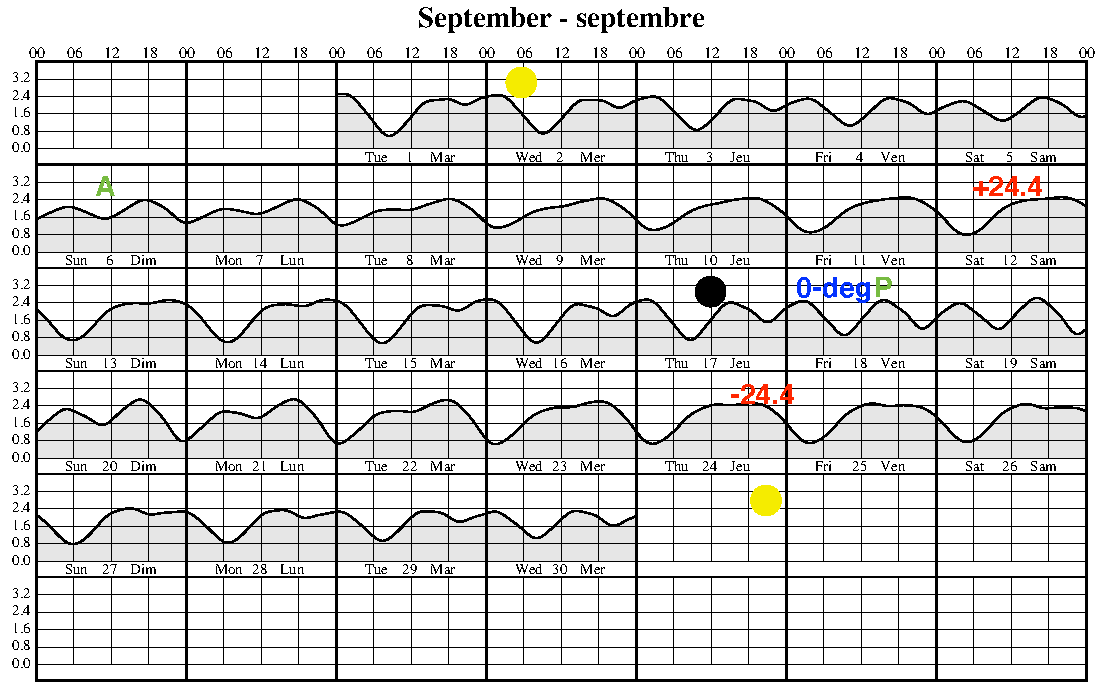
\includegraphics[width=3.7in]{figs/Waves/TideSep2020}
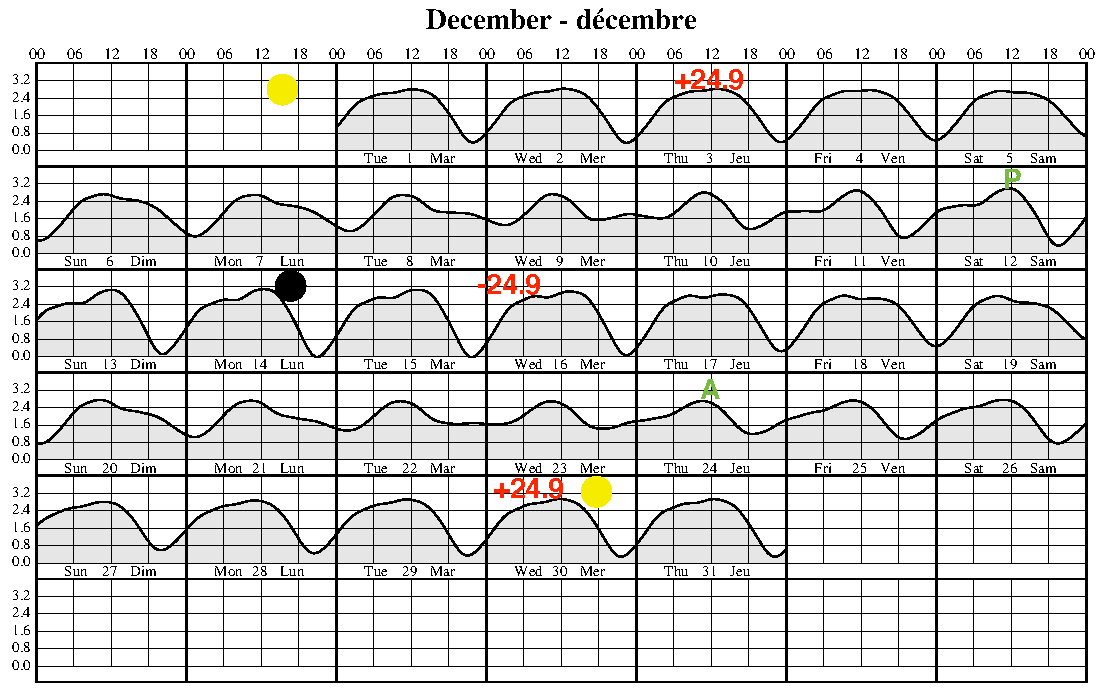
\includegraphics[width=3.7in]{figs/Waves/TideDec2020}    
\end{center}

Using what you learned in this chapter, describe as many features of the tides at Victoria as possible by comparing and contrasting the months, and the lunar and solar orbit characteristics.
 
%%% Local Variables:
%%% mode: latex
%%% TeX-master: t
%%% End:
